\documentclass[10pt, oneside]{article} 
\usepackage{amsmath, amsthm, amssymb, calrsfs, wasysym, verbatim, bbm, color, graphics, geometry}
\usepackage{graphicx}
\usepackage{float}
\usepackage{longtable}
\usepackage{rotating}
\usepackage{adjustbox}
\usepackage{booktabs}
\usepackage{caption}
\usepackage[english]{babel}
\usepackage[utf8]{inputenc}
\usepackage[table]{xcolor}
\usepackage{multicol}
\usepackage{hyperref}

\geometry{tmargin=.75in, bmargin=.75in, lmargin=.75in, rmargin = .75in}  

\newcommand{\R}{\mathbb{R}}
\newcommand{\C}{\mathbb{C}}
\newcommand{\Z}{\mathbb{Z}}
\newcommand{\N}{\mathbb{N}}
\newcommand{\Q}{\mathbb{Q}}
\newcommand{\Cdot}{\boldsymbol{\cdot}}

\newtheorem{thm}{Theorem}
\newtheorem{defn}{Definition}
\newtheorem{conv}{Convention}
\newtheorem{rem}{Remark}
\newtheorem{lem}{Lemma}
\newtheorem{cor}{Corollary}


\title{Computing Infrastructure: [Course Code]}
\author{[Sofia Martellozzo]}
\date{Academic Year 2021-2022}

\begin{document}

\maketitle
\newpage
\tableofcontents

\vspace{.25in}
\newpage

\section{Computing Infrastructure}

\subsection{Introduction}
\begin{defn}
{\bf Computing Infrastructure}: Technological infrastructure that provides hardware and software for computation to other systems and services.
\end{defn}


\begin{figure}[H]
    \begin{center}
    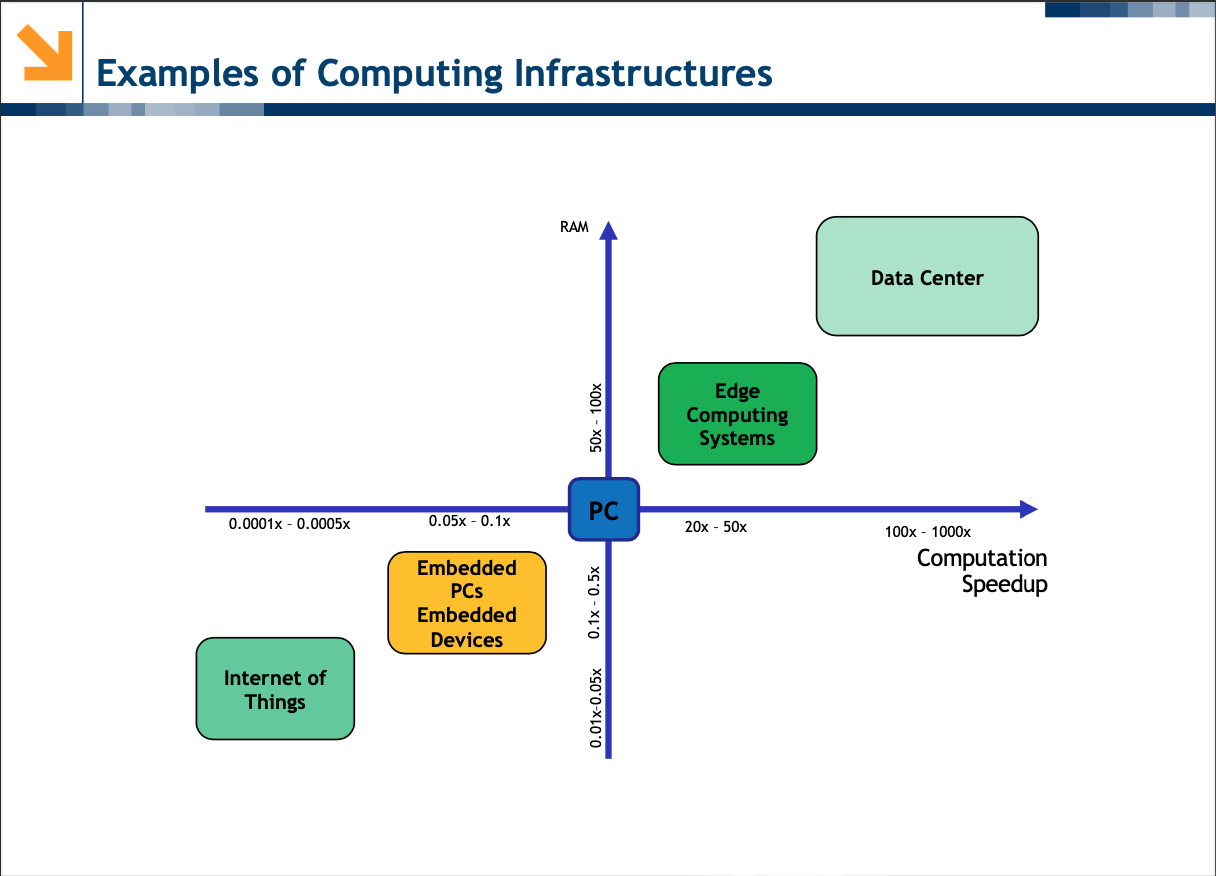
\includegraphics[width=0.5\textwidth]{img/img1.png}
    \caption{Computing Infrastructure}
    \label{fig:computing infrastructure}
    \end{center}
\end{figure}

\begin{multicols}{2}
{\bf Advantages}:
\begin{itemize}
    \item Lower IT costs
    \item High performance
    \item Instant software updates
    \item “Unlimited” storage capacity
    \item Increased data reliability
    \item Universal document access
    \item Device Independence 
\end{itemize}

\columnbreak

{\bf Disadvantages}:
\begin{itemize}
    \item Require a constant Internet connection
    \item Do not work well with low-speed connections
    \item Hardware Features might be limited
    \item Privacy and security issues
    \item High Power Consumption (1\% overall worldwide total energy consumption due to datacenters)
    \item Latency in making decision
\end{itemize}

\end{multicols}


\begin{figure}[H]
    \begin{center}
    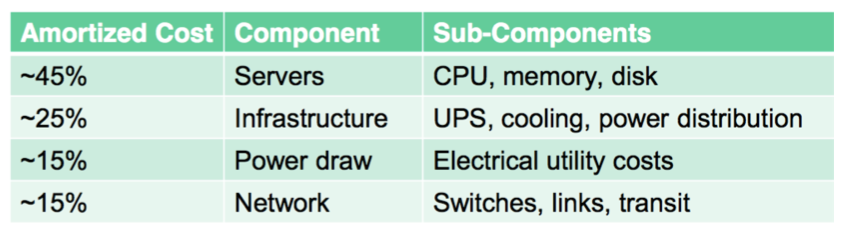
\includegraphics[width=0.5\textwidth]{img/img2.png}
    \label{fig:consumptions}
    \end{center}
\end{figure}

\newpage

%------------------------------------------------------%
\section{Data WareHouse}

\subsection{Introduction}
In the last few decades, computing and storage have moved from PC- like clients to smaller, often mobile, devices, combined with large internet services.\\
Traditional enterprises are also shifting to Cloud computing.
\begin{figure}[H]
    \begin{center}
    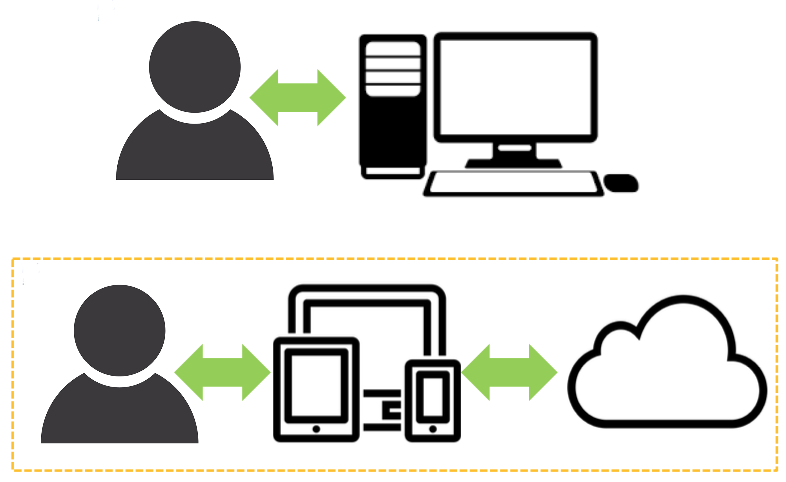
\includegraphics[width=0.5\textwidth]{img/img3.png}
    \label{fig:computing and storage}
    \end{center}
\end{figure}

\begin{multicols}{3}
{\bf User experience improvements}
\begin{itemize}
    \item Ease of management (no configuration or backups needed)
    \item Ubiquity of access
\end{itemize}

\columnbreak

{\bf Advantages to vendors}
\begin{itemize}
    \item Software-as-a-service allows faster application development (easier to make changes and improvements)
    \item Improvements and fixes in the software are easier inside their data centers (instead of updating many millions of clients with peculiar hardware and software configurations)
    \item The hardware deployment is restricted to a few well-tested configurations.
\end{itemize}

\columnbreak

{\bf Server-side computing allows}
\begin{itemize}
    \item Faster introduction of new hardware devices (e.g., HW accelerators or new hardware platforms)
    \item Many application services can run at a low cost per user.
\end{itemize}

\end{multicols}
Some workloads require so much computing capability that they are a more natural fit in datacenter (and not in client-side computing).\\
A couple of examples (Search services (web, images, and so on), Machine and Deep Learning (\href{https://www.theguardian.com/commentisfree/2020/sep/08/robot-wrote-this-article-gpt-3}{GPT-3}).

\subsection{From Data Centers to Warehouse-scale computers}
{\bf Data centers} = is a place in which there are many servers\\
{\bf Whareouse} = is a type of Data Center, it works as a computer.\\
The trends toward server-side computing and widespread internet services created a new class of computing systems:
\begin{defn}
{\bf warehouse-scale computers (WSCs)}The massive scale of the software infrastructure, data repositories, and hardware platform.
\begin{itemize}
    \item is an internet service (= service provided by inyternet)
    \item may consist of tens or more individual programs (= not a single program, a collection of them that together create/provide the service)
    \item such programs interact to implement complex end-user services such as email, search, maps or machine learning.
\end{itemize}
\end{defn}
Data centers are buildings where multiple servers and communication units are co-located because of their common environmental requirements and physical security needs, and for ease of maintenance.\\
In {\bf Traditional Data Center}: typically host a large number of relatively small- or medium-sized applications, each applications is running on a dedicated hardware infrastructure that is de-coupled and protected from other systems in the same facility, applications tend not to communicate each other. Those data centers host hardware and software for multiple organizational units or even different companies.
\begin{figure}[H]
    \begin{center}
    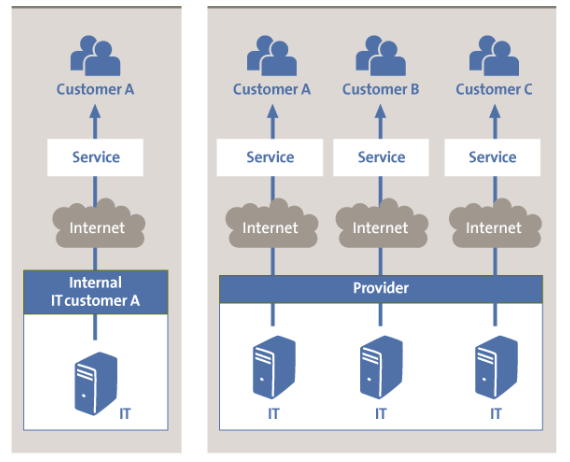
\includegraphics[width=0.3\textwidth]{img/img4.png}
    \caption{Traditional Data Center}
    \label{fig:Traditional Data Center}
    \end{center}
\end{figure}
{\bf WSCs} belong to a single organization, use a relatively homogeneous hardware and system software platform (=> easier to manage and cheaper, but has limitations on functionalities), and share a common systems management layer (such as Google, Facebook, Alibaba, Amazon, Dropbox...).\\
(you have 1 services that you want to provide to a 'huge' amount of customers)\\
Run a smaller number of very large applications (or internet services).\\
The common resource management infrastructure allows significant deployment flexibility.\\
The requirements of:
\begin{itemize}
    \item homogeneity
    \item single-organization control
    \item cost efficiency
\end{itemize}
\begin{figure}[H]
    \begin{center}
    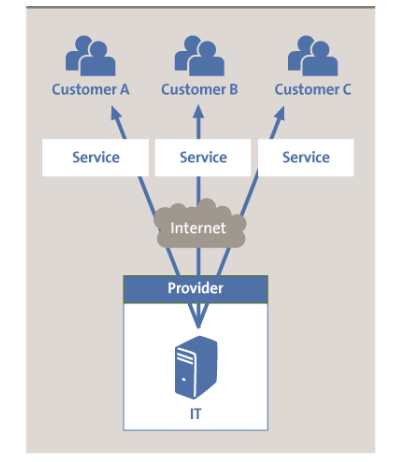
\includegraphics[width=0.25\textwidth]{img/img5.png}
    \caption{Warehouse-Scale Computers}
    \label{fig:WSCs}
    \end{center}
\end{figure}
Initially designed for online data-intensive web workloads, WSCs also now power public clouds computing systems (e.g., Amazon, Google, Microsoft). Such public clouds do run many small applications, like a traditional data center. (All of these applications rely on Virtual Machines (or Containers), and they access large, common services for block or database storage, load balancing, and so on, fitting very well with the WSC model).\\
These are not just a collection of servers: \\The software running on these systems executes on clusters of hundreds to thousands of individual servers (far beyond a single machine or a single rack)\\
+ \\The machine is itself this large cluster or aggregation of servers and needs to be considered as a single computing unit. (=> scale up in terms of performance)\\
{\bf Several datacenters}:
Multiple Data Center located far apart (placed near point of iterest) => becomes important also the PRIVACY: data of a country must remain in it.\\
Multiple data centers are (often) replicas of the same service (to reduce user {\bf latency} and improve serving {\bf throughput}).\\
A request is typically fully processed within one data center.\\
{\bf Availability}:
Services provided through WSCs must guarantee high availability, typically aiming for at least 99.99\% uptime (i.e., one-hour downtime per year). Achieving such fault-free operation is difficult when a large collection of hardware and system software is involved.\\
WSC workloads must be designed to gracefully tolerate large numbers of component faults with little or no impact on service level performance and availability.

\subsection{Architectural Overview of WSCs}
Hardware implementation of WSCs might differ significantly each other; However, the architectural organization of these systems is relatively stable.
\begin{figure}[H]
    \begin{center}
    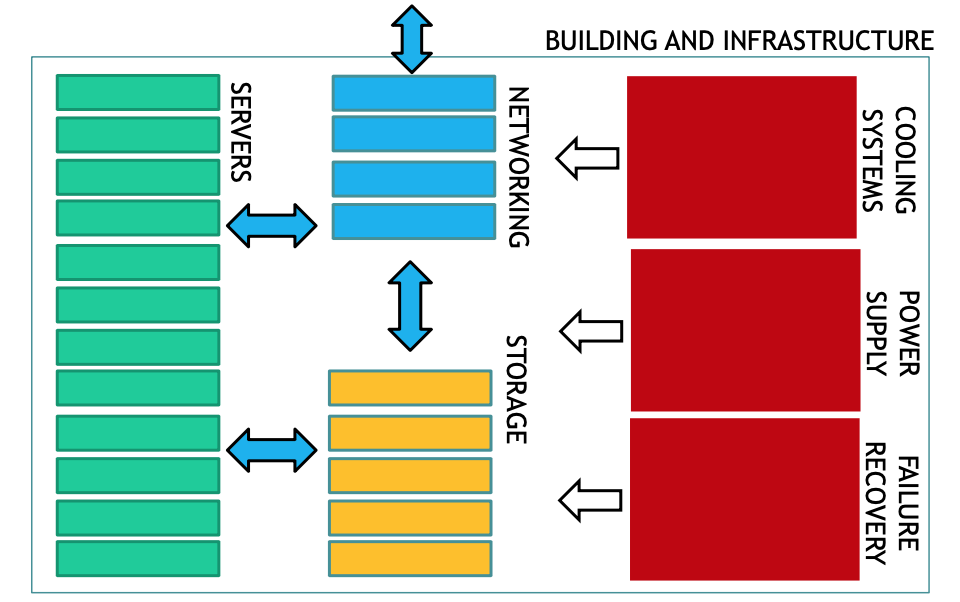
\includegraphics[width=0.4\textwidth]{img/img6.png}
    \caption{Warehouse-Scale Computers Overview}
    \label{fig:WSCs overview}
    \end{center}
\end{figure}




\newpage

%------------------------------------------------------%





\end{document}
